% !TEX root = ../FundationsDataScience.tex

\chapter{Deep Learning}
\label{c-deep-learning}

% Ref: \cite{Rufflewind2017blog}


%%%%%%%%%%%%%%%%%%%%%%%%%%%%%%%%%%%%%%%%%%%%%%%%%%%%%%%%%%%%%%%%%%%%%%%%
%%%%%%%%%%%%%%%%%%%%%%%%%%%%%%%%%%%%%%%%%%%%%%%%%%%%%%%%%%%%%%%%%%%%%%%%
%%%%%%%%%%%%%%%%%%%%%%%%%%%%%%%%%%%%%%%%%%%%%%%%%%%%%%%%%%%%%%%%%%%%%%%%
\section{Deep Architectures}
\label{sec-deepnet-discr}

%%%%%%%%%%%%%%%%%%%%%%%%%%%%%%%%%%%%%%%%%%
\subsection{Deep Network Structure}
\label{sec-deep-structure}

Deep learning are estimator $f(x,\be)$ which are built as composition of simple building blocks.
%
The inner layers can be understood as computing a lifted representation (feature map) of the input, while the last layer is a classical linear model (e.g. logistic classification). The difference with kernel method is that the feature map is not fixed but is learned from the data. 

%%%
\paragraph{Feedforward architectures.}

In their simplest form (non-recursive), they corresponds to a simple linear computational graph as already defined in~\eqref{eq-simple-lin-dag} (without the loss $\Ll$). Initialized as $x_0=x$, one computed
\eq{
	x_{\ell+1} = f_\ell(x_\ell,\be_\ell),  
}
so that $x_L=f(x,\be)$ with 
\eq{
	f(\cdot,\be) = f_{L-1}(\cdot,\be_{L-1}) \circ f_{L-2}(\cdot,\be_2) \circ \ldots \circ f_{0}(\cdot,\be_0)
}
where $\be=(\be_0,\ldots,\be_{L-1})$ is the set of parameters, and 
\eq{
	f_{\ell}(\cdot,\be_\ell) : \RR^{n_\ell} \rightarrow \RR^{n_{\ell+1}}.
}
%
While it is possible to consider more complicated computational graph (in particular recurrent ones, where the weight are shared by the functions), we restrict here out attention to these simple linear graph computation structures (so-called feedforward networks).

The supervised learning of these parameters $\be$ is usually done by empirical risk minimization~\eqref{eq-erm-param} using SGD-type methods as explained in Section~\ref{sec-stochastic-optim}. Note that this results in highly non-convex optimization problems. In particular, strong convergence guarantees such as Theorem~\ref{thm-conv-sgd} do not hold anymore, and only weak convergence (toward stationary points) holds. SGD type technics are however found to work surprisingly well in practice, and it now believe that the success of these deep-architecture approaches (in particular the ability of these over-parameterized model to generalize well) are in large part due to the dynamics of the SGD itself, which induce an implicit regularization effect. 

For these simple linear architectures, the gradient of the ERM loss~\eqref{eq-grad-formula} can be computed using the reverse mode computation detailed in Section~\ref{sec-reversemode-simple}. In particular, in the context of deep learning, formula~\eqref{eq-backprop}. One should however keep in mind that for more complicated (e.g. recursive) architectures, such a simple formula is not anymore available, and one should resort to reverse mode automatic differentiation (see Section~\ref{sec-reverse-mode}), which, while being conceptually simple, is actually implementing possibly highly non-trivial and computationally optimal recursive differentiation. 

%%%
\paragraph{Deep MLP.}

In most successful applications of deep-learning, each computational block $f_{\ell}(\cdot,\be_\ell)$ is actually very simple, and is the composition of 
\begin{rs}
	\item an affine map, $B_\ell \cdot + b_\ell$ with a matrix $B_\ell \in \RR^{n_\ell \times \tilde n_{\ell}}$ and a vector $b_\ell \in \RR^{\tilde n_\ell}$ parametrized (in most case linearly) by $\be_\ell$, 
	\item a fixed (not depending on $\be_\ell$) non-linearity $\rho_\ell : \RR^{\tilde n_{\ell}} \rightarrow \RR^{n_{\ell+1}}$
\end{rs}
which we write as
\eql{\label{eq-struc-layer}
	\foralls x_\ell \in \RR^{n_\ell}, \quad
	f_{\ell}(x_\ell,\be_\ell) = \rho_\ell(  B_\ell x_\ell + b_\ell ) \in \RR^{n_{\ell+1}}. 
}
In the simplest case, the so-called ``fully connected'', one has $(B_\ell,b_\ell)=\be_\ell$, i.e. $B_\ell$ is a full matrix and its entries (together with the bias $b_\ell$) are equal to the set of parameters $\be_\ell$. 
%
Also in the simplest cases $\rho_\ell$ is a pointwise non-linearity $\rho_\ell(z)=(\tilde\rho_\ell(z_k))_k$, where $\tilde\rho_\ell : \RR \rightarrow \RR$ is non-linear. The most usual choices are the rectified linear unit (ReLu) $\tilde\rho_\ell(s)=\max(s,0)$ and the sigmoid $\tilde\rho_\ell(s)=\th(s) = (1+e^{-s})^{-1}$.

The important point here is that the interleaving of non-linear map progressively increases the complexity of the function $f(\cdot,\be)$.

The parameter $\be = (B_\ell,b_\ell)_\ell$ of such a deep network are then trained by minimizing the ERM functional~\eqref{eq-erm-param} using SGD-type stochastic optimization method. The gradient can be computed efficiently (with complexity proportional to the application of the model, i.e. $O(\sum_\ell n_\ell^2)$) by automatic differentiation. Since such models are purely feedforward, one can directly use the back-propagation formula~\eqref{eq-simple-lin-dag}.

For regression tasks, one can can directly use the output of the last layer (using e.g. a ReLu non-linearity) in conjunction with a $\ell^2$ squared loss $L$.
%
For classification tasks, the output of the last layer needs to be transformed into class probabilities by a multi-class logistic map~\eqref{eq-multiclass-logitmap}.

An issue with such a fully connected setting is that the number of parameters is too large to be applicable to large scale data such as images. Furthermore, it ignores any prior knowledge about the data, such as for instance some invariance. This is addressed in more structured architectures, such as for instance convolutional networks detailed in Section~\ref{sec-cnn}. 


\begin{figure}
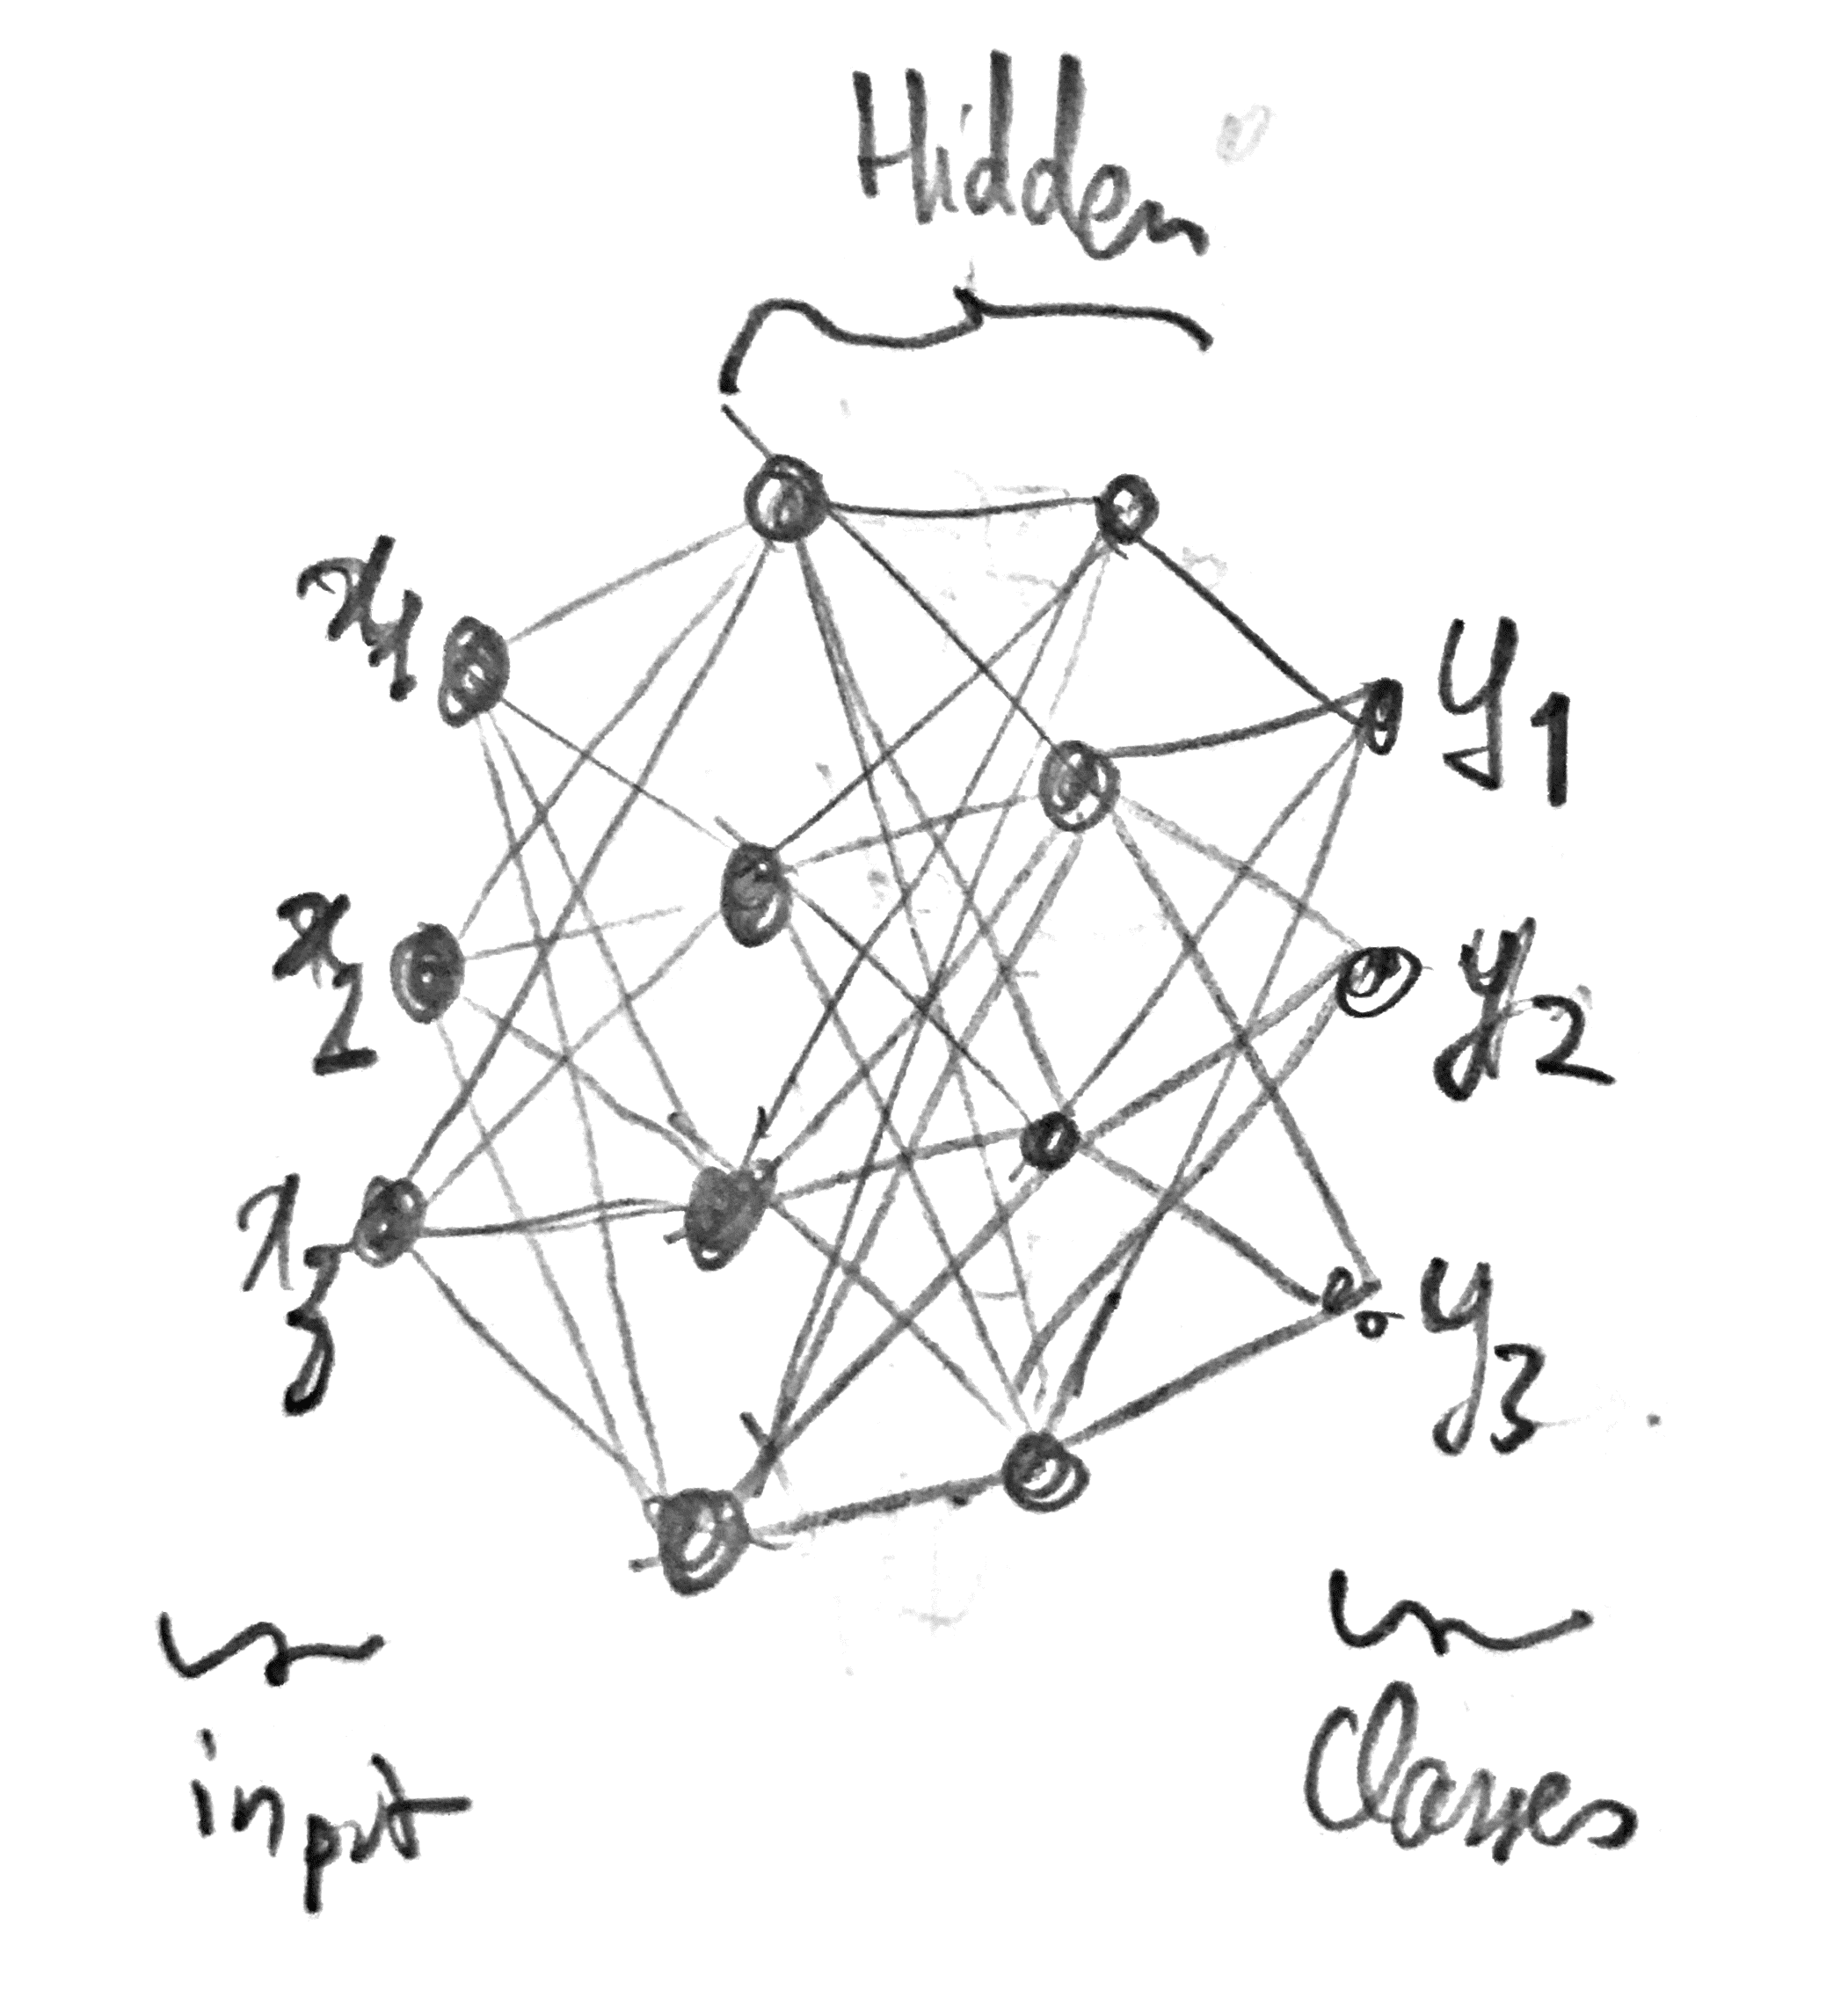
\includegraphics[width=.3\linewidth]{deep-learning/fc} \quad
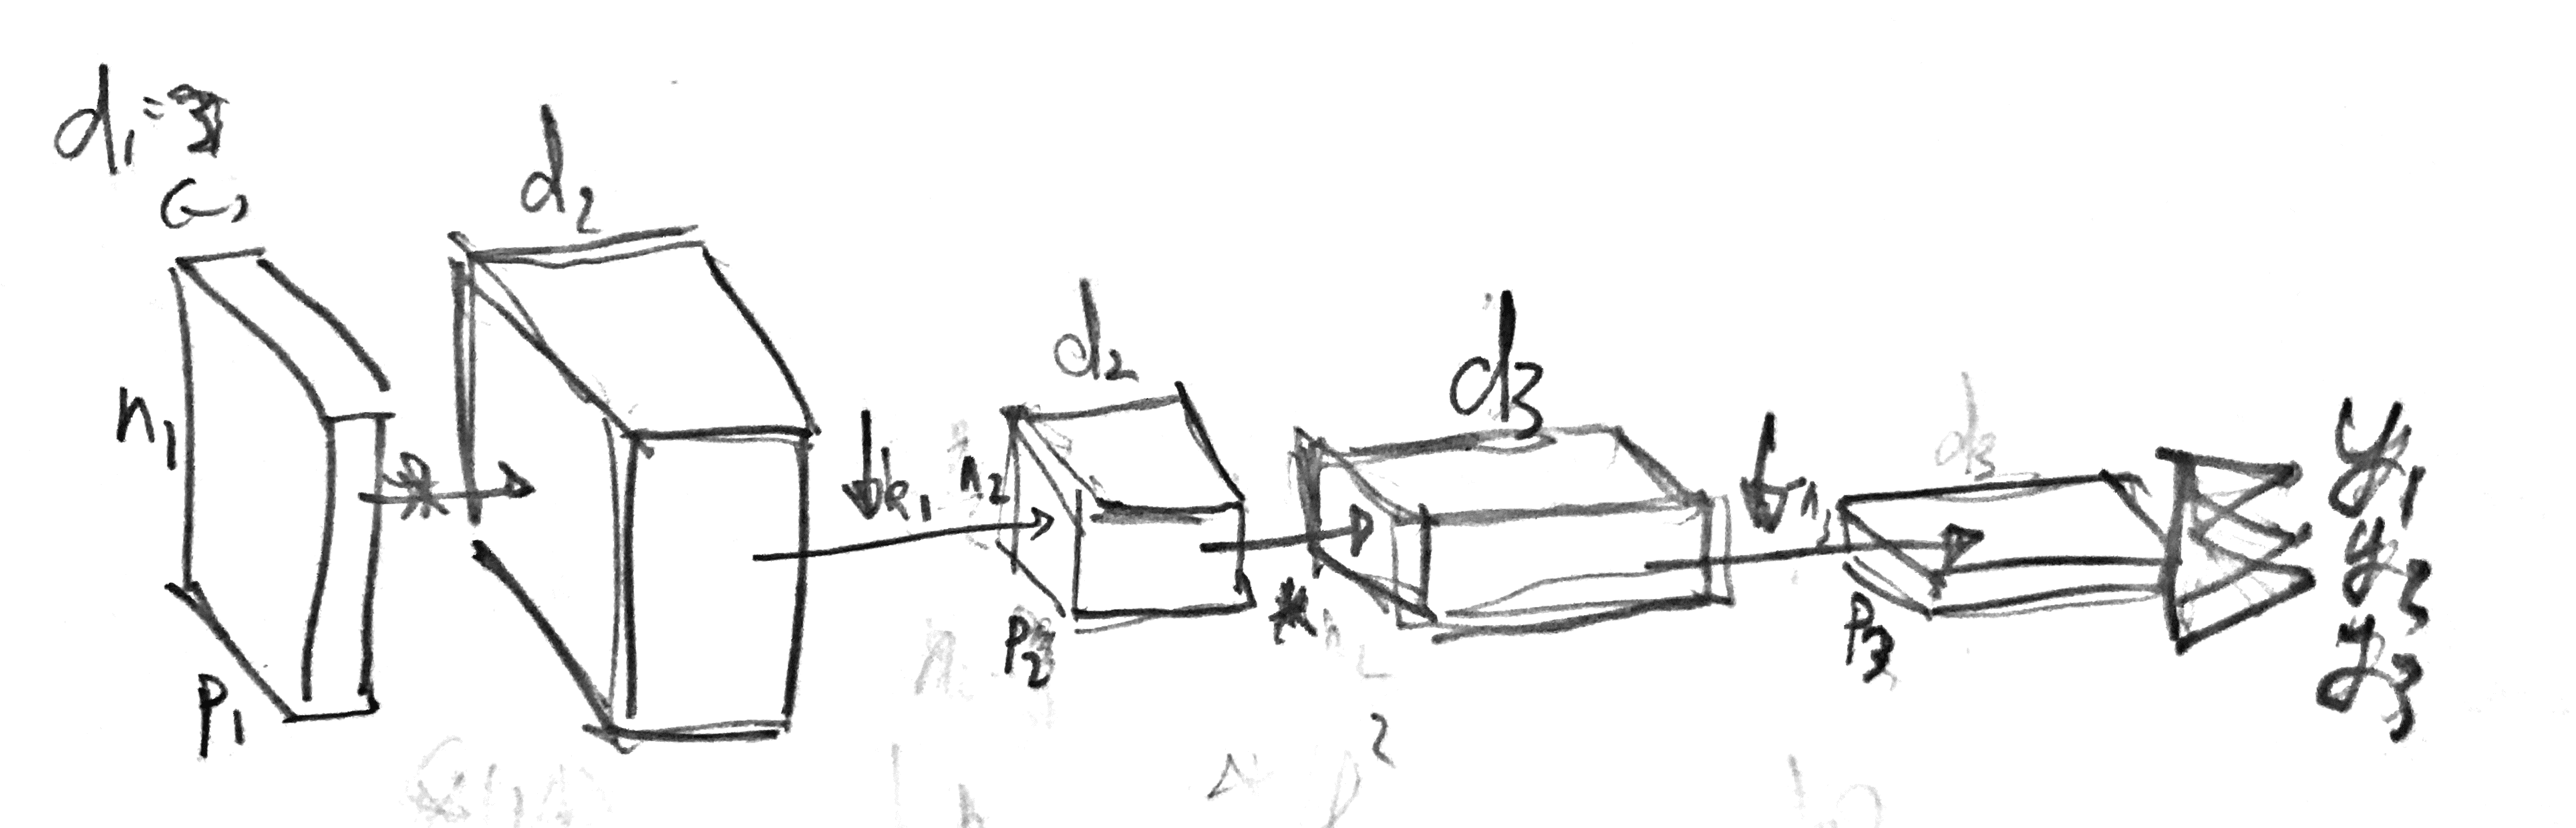
\includegraphics[width=.6\linewidth]{deep-learning/cnn}
\caption{\label{fig-bgd}
Left: example of fully connected network.
Right: example of convolutional neural network.
}
\end{figure}


%%%%%%%%%%%%%%%%%%%%%%%%%%%%%%%%%%%%%%%%%%
\subsection{Perceptron and Shallow Models}

Before going on with the description of deep architectures, let us re-interpret the logistic classification method detailed in Sections~\ref{sec-two-class-logit} and~\ref{sec-multiclass-logit}.

The two-class logistic classification model~\eqref{eq-two-class-logit-model} is equal to a single layer ($L=1$) network of the form~\eqref{eq-struc-layer} (ignoring the constant bias term) where 
\eq{
	B_0 x = \dotp{x}{\be}
	\qandq
	\tilde\rho_0(u) = \th(u).
}
The resulting one-layer network $f(x,\be) = \th(\dotp{x}{\be})$ (possibly including a bias term by adding one dummy dimension to $x$) is trained using the loss, for binary classes $y \in \{0,1\}$ 
\eq{
	L(t,y) = -\log( t^{y} (1-t)^{1-y} ) = -y\log(t)-(1-y)\log(1-t).
}
In this case, the ERM optimization is of course a convex program. 

Multi-class models with $K$ classes are obtained by computing $B_0 x = (\dotp{x}{\be_k})_{k=1}^K$, and a normalized logistic map 
\eq{
	f(x,\be) = \Nn( ( \exp(\dotp{x}{\be_k}) )_k )
	\qwhereq
	\Nn(u) = \frac{u}{\sum_{k} u_{k}}
} 
and assuming the classes are represented using vectors $y$ on the probability simplex, one should use as loss
\eq{
	L(t,y) = -\sum_{k=1}^K y_k \log(t_k). 
}

%%%%%%%%%%%%%%%%%%%%%%%%%%%%%%%%%%%%%%%%%%
\subsection{Convolutional Neural Networks}
\label{sec-cnn}

In order to be able to tackle data of large size, and also to improve the performances, it is important to leverage some prior knowledge about the structure of the typical data to process. For instance, for signal, images or videos, it is important to make use of the spacial location of the pixels and the translation invariance (up to boundary handling issues) of the domain.

Convolutional neural networks are obtained by considering that the manipulated vectors $x_\ell \in \RR^{n_\ell}$ at depth $\ell$ in the network are of the form $x_\ell \in \RR^{ \bar n_\ell \times d_\ell }$, where $\bar n_\ell$ is the number of ``spatial'' positions (typically along a 1-D, 2-D, or 3-D grid) and $d_\ell$ is the number of ``channels''.
%
For instance, for color images, one starts with $\tilde n_\ell$ being the number of pixels, and $d_\ell=3$.
%
To ease the writing, we denote $x_\ell = ( (x_\ell)_r[i] )_{r,i}$ where $i \in \{1,\ldots,\bar n_\ell\}$ is the pixel location, and $r \in \{1,\ldots,d_\ell\}$ is the channel index.

The linear operator $B_\ell : \RR^{ \bar n_\ell \times d_\ell } \rightarrow \RR^{ \bar n_\ell \times d_{\ell+1} }$ is then (up to boundary artefact) translation invariant and hence a convolution along each channel (note that the number of channels can change between layers). This is formalized in the following proposition.

\begin{prop}
	Let $B : \RR^{n \times d} \rightarrow \RR^{n \times d'}$ (where $n$ indicates ``spacial'' dimension, with periodic boundary conditions). Then $x = (x_r[i] )_{r,i} \mapsto B x$ is co-variant with translation, i.e. 
	\eq{
		\foralls \tau, \quad
		B (x[\cdot-\tau]) = (B x)[\cdot-\tau]
	}
	(one translate the pixels) if and only if there exists a set of filters $\psi = ( \psi_{r,s} \in \RR^n )_{r=1,\ldots,d}^{s=1,\ldots,d'}$ such that 
	\eql{\label{eq-structure-convolution}
		\foralls r=1,\ldots,d', \quad
		(B x)_{r} = \sum_{s=1}^{d} \psi_{r} \star x_{s}
	}
	\eq{
		\text{i.e.} \quad
		(B x)_{r}[i] = \sum_{s=1}^{d} \sum_j \psi_{r,s}[i-j] \star x_{s}[j]
	}	
	where $\star$ is the convolution on $\RR^n$ (for instance 1-D or 2-D convolution). 
\end{prop}

\begin{proof}
	Since convolutions are covariant with translation on $\RR^n$, formula~\eqref{eq-structure-convolution} defines covariant operators.
	%
	We now assume $B$ is covariant. We define $\de^{s}$ the dirac at pixel $i=0$ and channel $s$, i.e. $(\de^{s})_{s'}[i] = 1_{s=s'} 1_{i=0}$, and then we let $\tilde\psi_{r,s} \eqdef (B \de^s)_r$. One has the decomposition of a vector as translated Diracs
	\eq{
		x = \sum_{j,s} x_s[j] \de^s[\cdot-j], 
	}
	so that by linearity and translation co-variance
	\eq{
		(B x)_r = \sum_{j,s} x_s[j] (B \de^s[\cdot-j])_r
		=  \sum_{j,s} x_s[j] (B \de^s)_r[\cdot-j]
		=  \sum_{j,s} x_s[j] \tilde\psi_{r,s}[\cdot-j]
		= \sum_s \psi_{r,s} \star x_s
	}
	where $\psi_{r,s}[i] = \tilde \psi_{r,s}[-i]$ is the reversed filter. 
\end{proof}

Using this proposition, a covariant $B_\ell$  is thus parameterized by a set of filters $\psi_\ell = ( (\psi_\ell)_{r,s} )_{s=1,\ldots,d_{\ell}}^{r=1,\ldots,d_{\ell+1}}$. Denoting $x_\ell = ( (x_{\ell})_{\cdot,s} )_{s=1}^{d_\ell}$ the different layers composing $x_\ell$, the linear map reads
\eq{
	\foralls r \in \{1,\ldots,d_{\ell+1}\}, \quad
	(B_\ell x_\ell)_{r} = \sum_{s=1}^{d_\ell} (\psi_\ell)_{r,s} \star (x_{\ell})_{s}, 
}
and the bias term $(b_\ell)_{\cdot,r} = (\tilde b_\ell)_r \in \RR$ is contant across the spacial dimension (to maintain translation invariance).
%
Translation covariance results in a weight-sharing: all the neurons (associated to an output pixels) have the same weights, defined by $\psi_\ell$. 

The non-linear maps across layers serve two purposes: as before a point-wise non-linearity is applied, and then a sub-sampling helps to reduce the computational complexity of the network. This is very similar to the construction of the fast wavelet transform. Denoting by $m_k$ the amount of down-sampling, where usually $m_k=1$ (no reduction) or $m_k=2$ (reduction by a factor two in each direction). One has
\eq{
	\rho_\ell(u) = \pa{ \tilde \rho_\ell( u_{s}[m_k\cdot] ) }_{s=1\ldots,d_{\ell+1}}.
}
In the literature, it has been proposed to replace linear sub-sampling by non-linear sub-sampling, for instance the so-called max-pooling (that operate by taking the maximum among groups of $m_\ell$ successive values), but it seems that linear sub-sampling is sufficient in practice when used in conjunction with very deep (large $L$) architectures. 

The intuition behind such model is that as one moves deeper through the layers, the neurons are receptive to larger areas in the image domain (although, since the transform is non-linear, precisely giving sense to this statement and defining a proper ``receptive field'' is non-trivial). Using an increasing number of channels helps to define different classes of ``detectors'' (for the first layer, they detect simple patterns such as edges and corner, and progressively capture more elaborated shapes).

In practice, the last few layers (2 or 3) of such a CNN architectures are chosen to be fully connected. This is possible because, thanks to the sub-sampling, the dimension of these layers are small.  

The parameters of such a model are the filters $\be = ( (\psi_\ell){r,s})_{\ell,s,r}$, and they are trained by minimizing the ERM functional~\eqref{eq-erm-param}. The gradient is typically computed by backpropagation. Indeed, when computing the gradient with respect to some filter $\psi_{\ell,r,s}$, the feedforward computational graph has the form~\eqref{eq-simple-lin-dag}. For simplicity, we re-formulate this computation in the case of a single channel per layer (multiple layer can be understood as replacing convolution by matrix-domain convolution). The forward pass computes all the inner coefficients, by traversing the network from $\ell=0$ to $\ell=L-1$, 
\eq{
	x_{\ell+1} = \rho_\ell(\psi_{\ell} \star x_\ell)
}
where $\rho_\ell(u)=(\tilde\rho_\ell(u_i))_i$ is applied component wise. Then, denoting $\Ee(\be) = \Ll( \be,y )$ the loss to be minimized with respect to the set of filters $\be=(\psi_\ell)_\ell$, and denoting $\nabla_\ell \Ee(\be) = \pd{\Ee( \be )}{\psi_\ell}$ the gradient with respect to $\psi_\ell$, one computes all the gradients by traversing the network in reverse order, from $\ell=L-1$ to $\ell=0$
\eql{\label{eq-backprop}
	\nabla_\ell \Ee(\be) = 
		[ \rho_\ell'(\psi_{\ell} \star x_\ell) ]
		\odot
		[ 
			\bar\psi_{\ell} \star \nabla_{\ell+1} \Ee(\be)
		], 
}
where $\rho_\ell'(u)=( \tilde\rho_\ell'( u_i ) )_i$ applies the derivative of $\tilde\rho_\ell$ component wise, and where $\bar \psi_{\ell} = \psi_\ell(-\cdot)$ is the reversed filter. Here, $\odot$ is the pointwise multiplication of vectors.
%
The recursion is initialized as $\nabla \Ee_L(\be) = \nabla \Ll(x_L,y)$, the gradient of the loss itself. 

This recursion~\eqref{eq-backprop} is the celebrated backpropagation algorithm put forward by Yann Lecun. Note that to understand and code these iterations, one does not need to rely on the advanced machinery of reverse mode automatic differentiation exposed in Section~\ref{sec-reverse-mode}. The general automatic differentiation method is however crucial to master because advanced deep-learning architectures are not purely feedforward, and might include recursive connexions. Furthermore, automatic differentiation is useful outside deep learning, and considerably eases prototyping for modern data-sciences with complicated non-linear models.  


%%%%%%%%%%%%%%%%%%%%%%%%%%%%%%%%%%%%%%%%%%
\subsection{Advanced Architectures}
\label{sec-advanced}


%%%
\paragraph{Residual Networks}

Residual network introduce so-called skip connexions of the form (for a significant sub-set of $\ell$)
\eq{
	f_\ell(x_\ell,\be_\ell) = x_\ell + \tilde f_\ell(x_\ell,\be_\ell)
}
where $\tilde f_\ell(\cdot,\be_\ell) : \RR^{n_\ell} \rightarrow \RR^{n_\ell}$ (the dimension is kept during these connexion). These connexion stabilize the training and enables the use of very deep network. They can also be interpreted as explicit Euler discretization of ODE's.
%
The usual choice for these layer is to have a bottleneck shape, of the form 
\eq{
	\tilde f_\ell(x_\ell,\be_\ell) = C_\ell^\top \rho_\ell( B_\ell x_\ell )
}
(ignoring biases) where $\be_\ell = (B_\ell, C_\ell) \in \RR^{m_\ell \times n_\ell} \times \RR^{m_\ell \times n_\ell}$ with $m_\ell \ll n_\ell$ to enforce a regularization effect. 


%%%
\paragraph{Batch normalization}

TODO write me.

%%%
\paragraph{Transformers Networks}

Transformers networks operates over distribution of points using a parametric push-forward of the point locations. They have a quadratic complexity in term of number of input points. 
%
The input $x$ of such a layer is a set of points $x = (x_i)_{i=1}^n$ where $x_i \in \RR^d$, and each point is modified as 
\eq{
	x_k \mapsto \sum_{i} \exp(-\dotp{Q x_i}{K x_k}) V x_i.
}
where $Q,K,V$ are the query, key and value matrices (which are the parameters of the layer). 

%%%%%%%%%%%%%%%%%%%%%%%%%%%%%%%%%%%%%%%%%%
\subsection{Scattering Transform}
\label{sec-scattering}

The scattering transform, introduced by Mallat and his collaborators, is a specific instance of deep convolutional network, where the filters $ (\psi_{\ell,r,s})_{\ell,s,r}$ are not trained, and are fixed to be wavelet filters. This network can be understood as a non-linear extension of the wavelet transform. In practice, the fact that it is fixed prevent it to be applied to arbitrary data (and is used mostly on signals and images) and it does not lead to state of the art results for natural images. Nevertheless, it allows to derives some regularity properties about the feature extraction map $f(\cdot,\be)$ computed by the network in term of stability to diffeomorphisms. It can also be used as a set of fixed initial features which can be further enhanced by a trained deep network, as shown by Edouard Oyallon.  

\if 0

%%%%%%%%%%%%%%%%%%%%%%%%%%%%%%%%%%%%%%%%%%%%%%%%%%%%%%%%%%%%%%%%%%%%%%%%
%%%%%%%%%%%%%%%%%%%%%%%%%%%%%%%%%%%%%%%%%%%%%%%%%%%%%%%%%%%%%%%%%%%%%%%%
%%%%%%%%%%%%%%%%%%%%%%%%%%%%%%%%%%%%%%%%%%%%%%%%%%%%%%%%%%%%%%%%%%%%%%%%
\section{Deep Generative Models}
\label{sec-deepnet-gen}


%%%%%%%%%%%%%%%%%%%%%%%%%%%%%%%%%%%%%%%%%%
\subsection{Density Fitting}

%%%
\paragraph{Fitting and MLE}

%%%
\paragraph{Generative Models}

%%%%%%%%%%%%%%%%%%%%%%%%%%%%%%%%%%%%%%%%%%
\subsection{Auto-encoders}

%%%%%%%%%%%%%%%%%%%%%%%%%%%%%%%%%%%%%%%%%%
\subsection{GANs}

\fi